\documentclass[12pt]{article}
% Эта строка — комментарий, она не будет показана в выходном файле
\usepackage{ucs}
\usepackage[warn]{mathtext}
\usepackage[utf8x]{inputenc} % Включаем поддержку UTF8
\usepackage[russian]{babel}  % Включаем пакет для поддержки русского языка
\usepackage{amsmath}
\usepackage{mathtools}
\usepackage{amssymb}
% \usepackage[dvips]{graphicx}
% \graphicspath{{noiseimages/}}
\usepackage[pdftex]{graphicx}


% Параметры страницы: 1см от правого края и 2см от остальных.


\hoffset=0mm
\voffset=0mm
\textwidth=180mm        % ширина текста
\oddsidemargin=-6.5mm   % левое поле 25.4 - 5.4 = 20 мм
\textheight=240mm       % высота текста 297 (A4) - 40
\topmargin=-15.4mm      % верхнее поле (10мм)
\headheight=5mm      % место для колонтитула
\headsep=5mm          % отступ после колонтитула
\footskip=8mm         % отступ до нижнего колонтитула

\begin{document}
	\author {Жарков Андрей 495}
	\title {Лабораторная работа 2.2.1 \\  Исследование затухающих колебаний в колебательном контуре.}
    \maketitle{}
	    
    \begin{center}
       	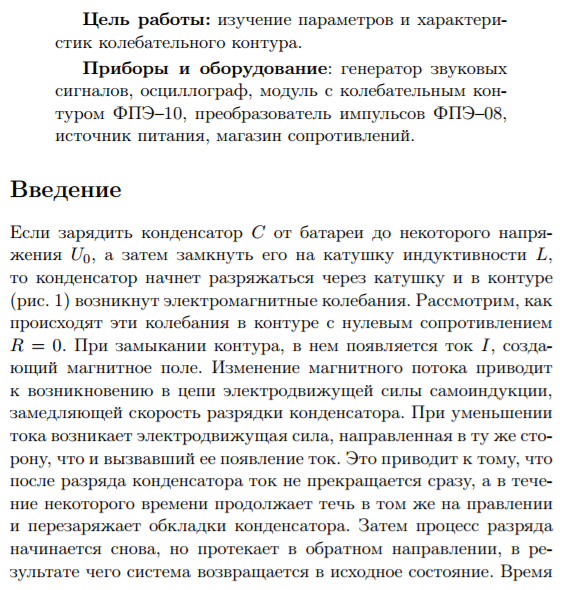
\includegraphics[width=15cm]{theory1.png}
       	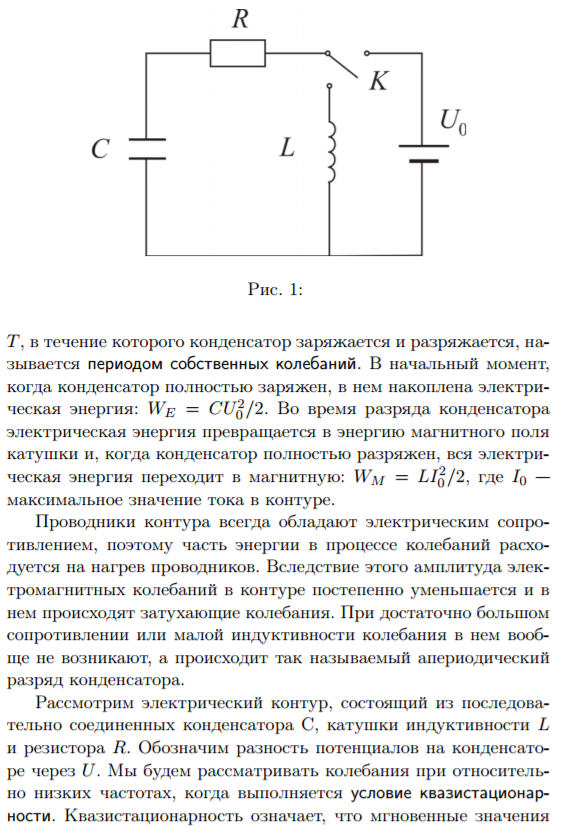
\includegraphics[width=15cm]{theory2.png}
       	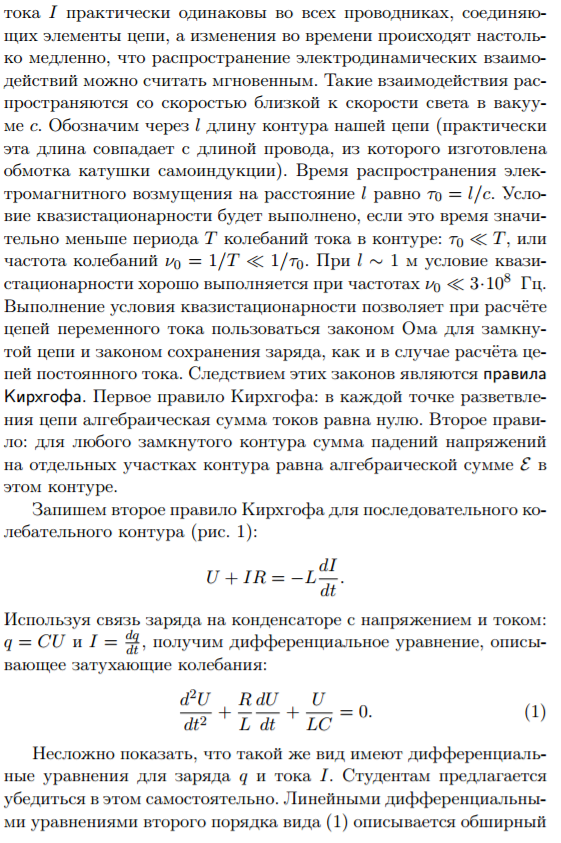
\includegraphics[width=15cm]{theory3.png}
       	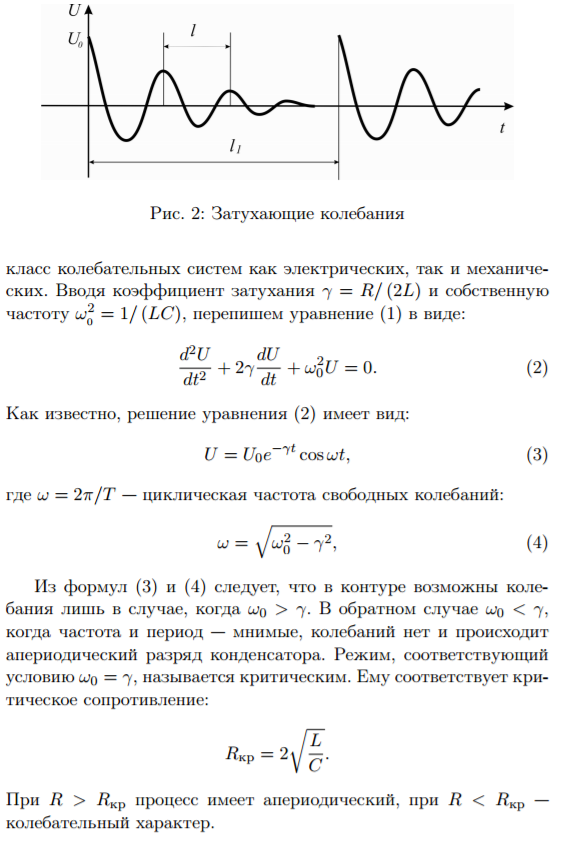
\includegraphics[width=15cm]{theory4.png}
       	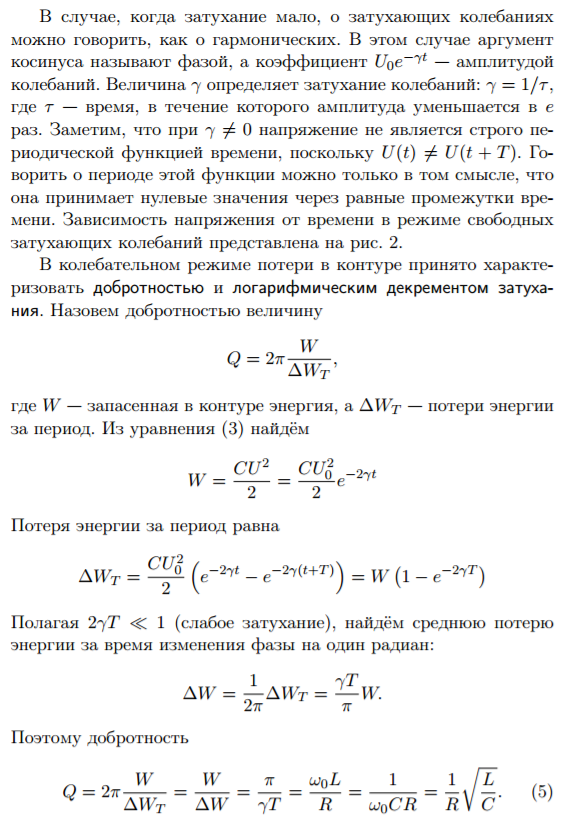
\includegraphics[width=15cm]{theory5.png}
        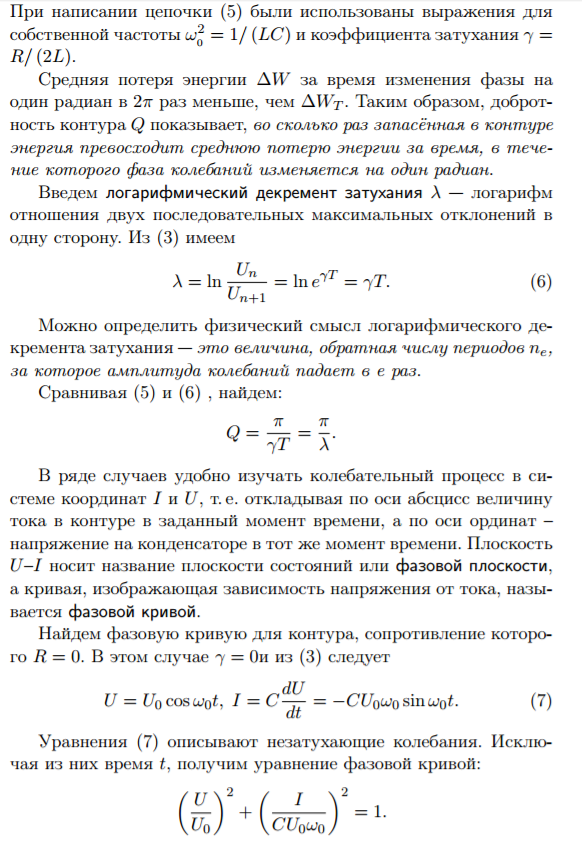
\includegraphics[width=15cm]{theory6.png}
	    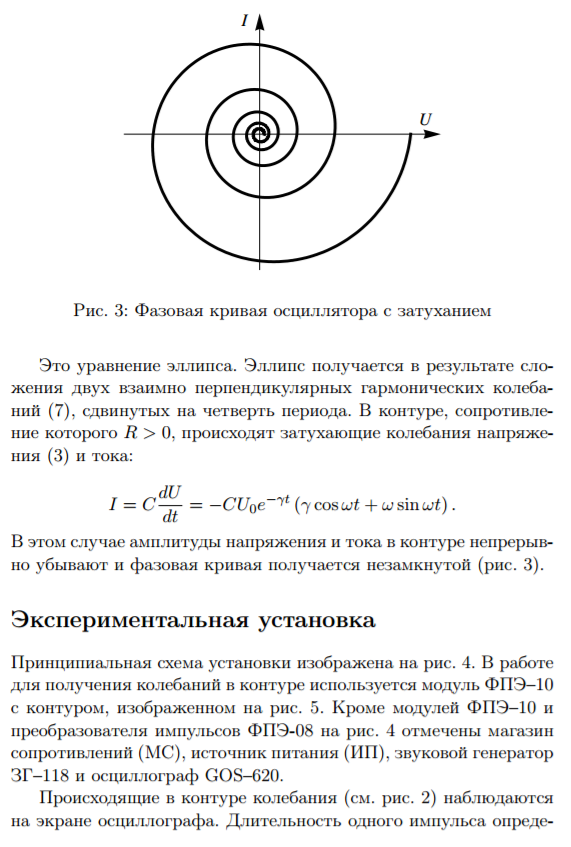
\includegraphics[width=15cm]{theory7.png}
	    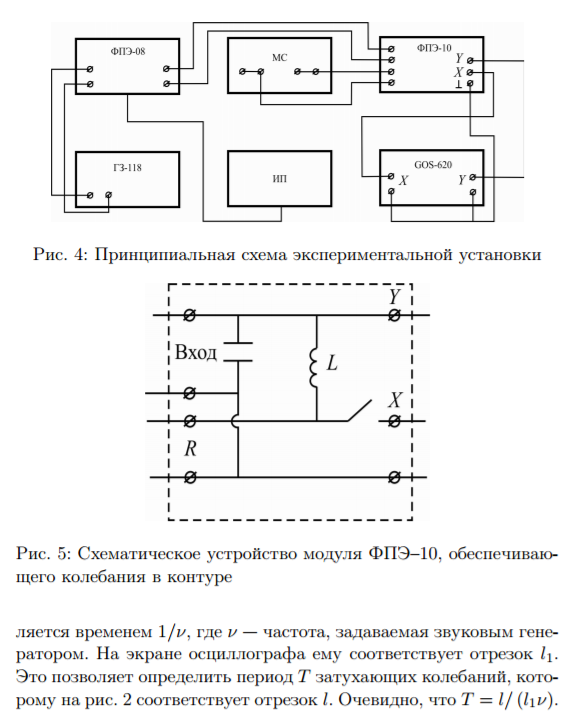
\includegraphics[width=15cm]{theory8.png}
    \end{center}
    
    \begin{center}
    	\textbf{\large Выполнение работы.}
    \end{center}
    
    Установим частоту звукового генератора $\nu = 250 Гц$.
    
    При различных сопротивлениях будем измерять расстояние $l$ (соответствующее периоду затухающих колебаний) и расстояние между цугами $l_1$ (соответствующее частоте, задаваемой звуковым генератором). Также измерим амплитуду двух последовательно идущих колебаний и вычислим логарифмический декремент затухания $\lambda = ln\frac{U_n}{U_{n+1}}$. После первых нескольких измерений, подтвердилось $\frac{U_n}{U_{n+1}} = \frac{U_k}{U_{k+1}}$, поэтому в таблице с измерениями указаны результаты только для двух последовательных измерений.
    
    \begin{center}
    	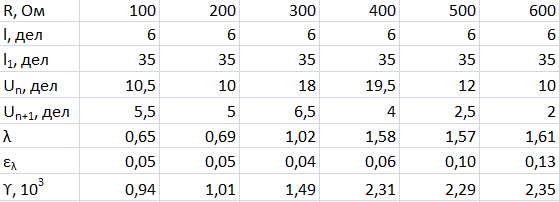
\includegraphics[width=15cm]{table1.png}
    \end{center}
    
    При измерениях, погрешность $\sigma = 0,25дел$.
    
    В таблице, коэффициент затухания $\gamma$ рассчитывался как $\frac{\lambda}{T}$. Как видно из таблицы, при всех сопротивлениях период $T$ получился один и тот же. $T = l/(l_1\nu) = 0,69 \pm 0,03 мс$
    
    Построим график $\lambda(R) = \frac{T}{2L}R + \frac{R_k T}{2L}$:
    
    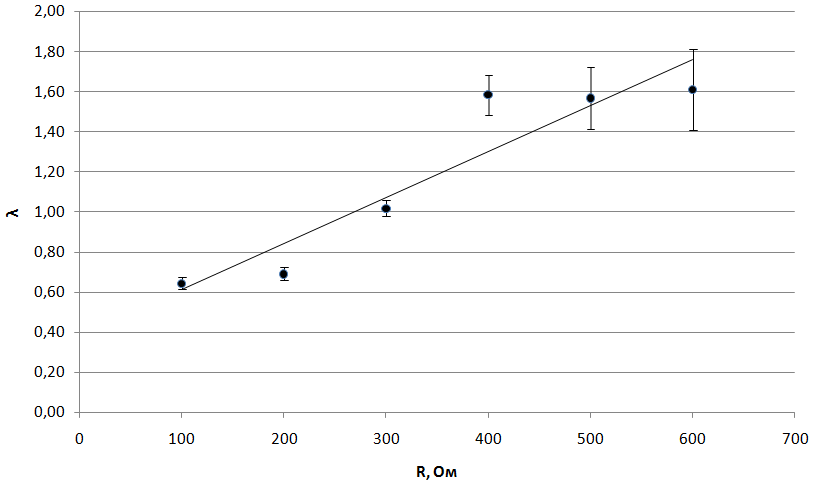
\includegraphics[width=15cm]{graph1.png}
    
    Найденные $k = (2,8 \pm 0,4) * 10^{-3} Ом^{-1}$, $b = 0,38 \pm 0,03$.
    
    Откуда находим $L = \frac{T}{2k} = 123 \pm 18 мГн$, $R_k = \frac{2Lb}{T} = 138 \pm 27 Ом$.
    
    Далее из $\frac{2\pi}{T} = \sqrt{\frac{1}{LC} - \gamma^2}$ получаем $C = \frac{T^2}{(\gamma^2T^2 + 4\pi^2)L} \approx \frac{T^2}{4\pi^2L} = 0,10 \pm 0,01 мкФ$
    
    Найденные значения в пределах погрешности совпадают с реальными параметрами установки $L = 100 \pm 5 мГн$, $C = 0,1 мкФ (\pm 10\%)$.
    
    Подберём сопротивление, при котором происходит апериодический разряд конденсатора. $R_{маг} = 1990 Ом$. Тогда $R = R_{маг} + R_k \approx 2120 Ом$. Теоретическая оценка $R_{кр} = 2\sqrt{\frac{L}{C}} = (2,2 \pm 3) * 10^3 Ом$. В пределах погрешности совпадают.
    
    \pagebreak
    
    Измерим амплитуду напряжений и токов, разделённых периодом времени (т. е. расстояния от центра фазовой кривой до точки пересечения витков спирали оси соответственно напряжения или тока).
    
    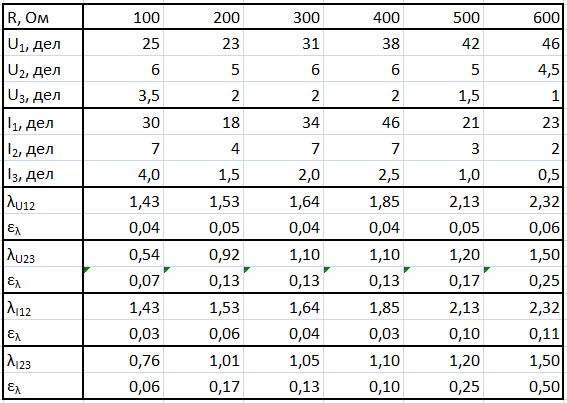
\includegraphics[width=15cm]{table2.png}
    
    Фазовая кривая при апериодическом разряде конденсатора:
    
    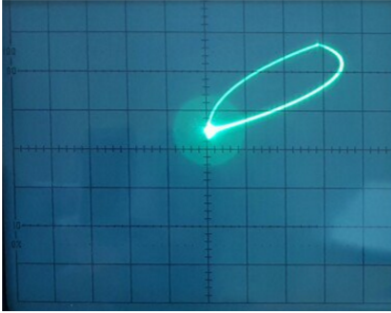
\includegraphics[width=5cm]{img.png}
    
    Теперь рассчитаем добротность контура Q для максимального и минимального значения $\lambda$:
    
    $Q_{min} = \frac{\pi}{\lambda_{min}} = 5,8 \pm 0,3$
    
    $Q_{min} = \frac{1}{R}\sqrt{\frac{L}{C}} = 5,5 \pm 0,6$
    
    $Q_{max} = \frac{\pi}{\lambda_{max}} = 1,35 \pm 0,07$
    
    $Q_{max} = \frac{1}{R}\sqrt{\frac{L}{C}} = 1,6 \pm 0,3$
    
    В пределах погрешности совпадают с теоретическими.
\end{document}